\documentclass[12pt]{beamer}

\usetheme[progressbar=frametitle]{metropolis}
\usepackage{appendixnumberbeamer}

\usepackage{booktabs}
\usepackage[scale=2]{ccicons}

\usepackage{pgfplots}
\usepgfplotslibrary{dateplot}

\usepackage{xspace}
\newcommand{\themename}{\textbf{\textsc{metropolis}}\xspace}

\title{How Faulting Keeps the Crust Strong}
\subtitle{Townend \& Zoback}
% \date{\today}
\date{}
\author{Prithvi Thakur}
\institute{Paper discussion}
% \titlegraphic{\hfill\includegraphics[height=1.5cm]{logo.pdf}}

\begin{document}

\maketitle

\begin{frame}[fragile]{Key Points}
    \begin{itemize}
        \item Intraplate crust: critically stressed, hydrostatic pore pressure, high permeability.
        \item Observed friction coefficient = 0.6-1.0. The theoretical friction coefficient for brittle rocks is 0.6.
        \item Laboratory measurements show upto four orders of magnitude lower permeability than in-site borehole measurements.
        \item Critically stressed rocks are hydraulically conductive.
    \end{itemize}
\end{frame}

\begin{frame}[fragile]{Key Points}
    \begin{itemize}
        \item Characteristic diffusion rate for fluid transport in the upper 1-10km is 10-1000 yr. 
        \item Intraplate crust is able to sustain higher differential stresses than would be possible if bulk permeability were sufficiently low to sustain fluid pressures higher than hydrostatic.
    \end{itemize}
\end{frame}

\begin{frame}[fragile]{Discussion}
    \begin{figure}
        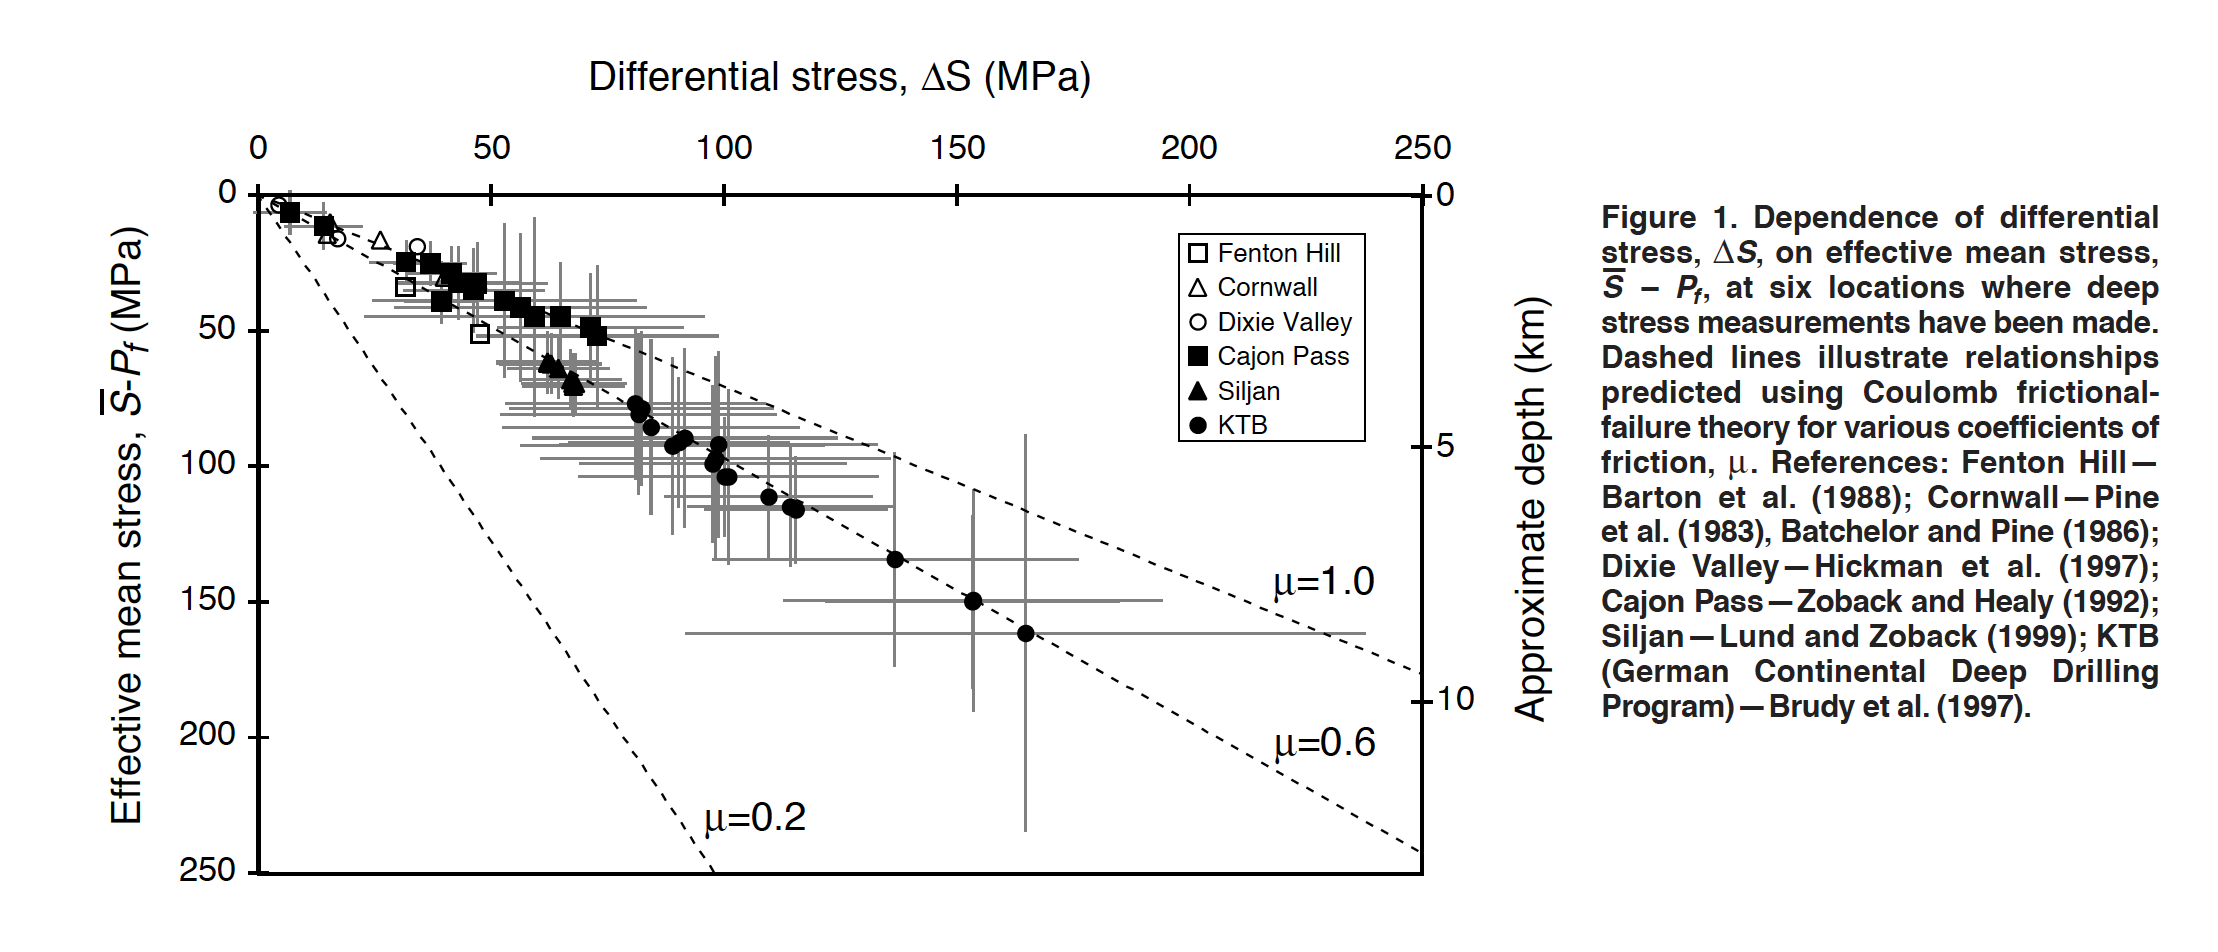
\includegraphics[width=1\linewidth]{images/1}
    \end{figure}
\end{frame}
\begin{frame}[fragile]{Discussion}
    \begin{figure}
        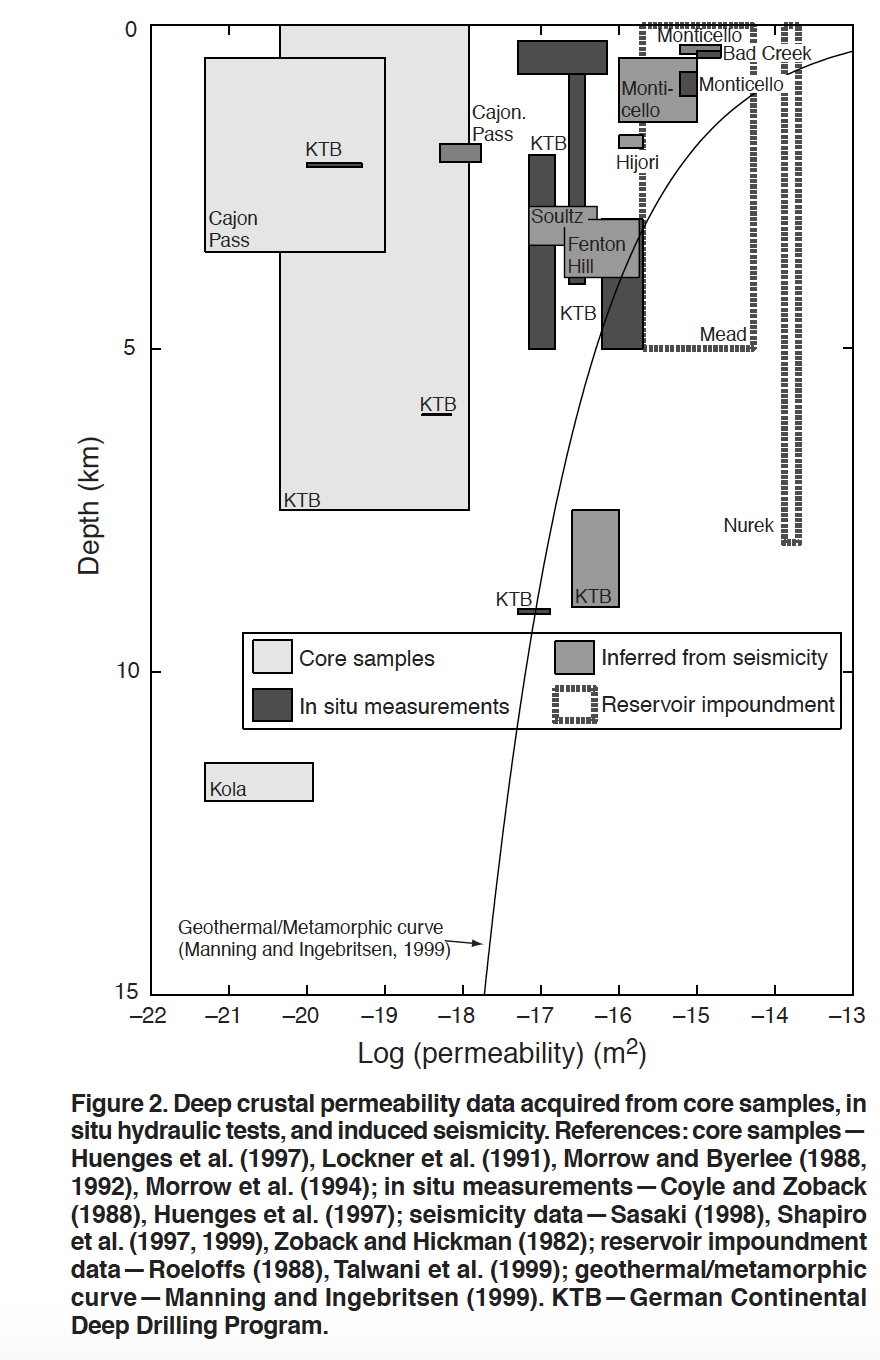
\includegraphics[width=0.48\linewidth]{images/2}
    \end{figure}
\end{frame}
\begin{frame}[fragile]{Discussion}
    \begin{figure}
        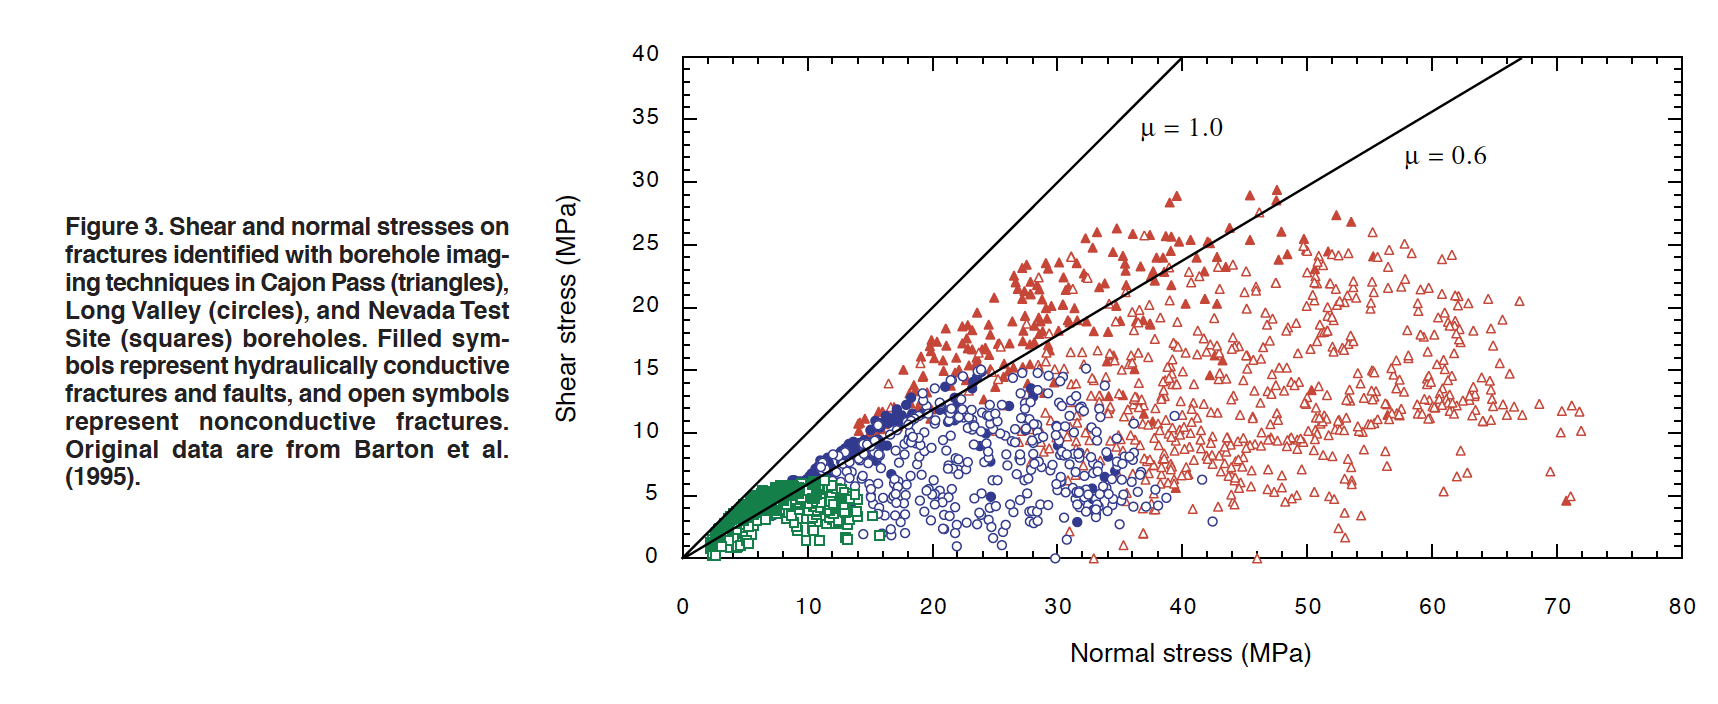
\includegraphics[width=1\linewidth]{images/3}
    \end{figure}
\end{frame}
\begin{frame}[fragile]{Discussion}
    \begin{figure}
        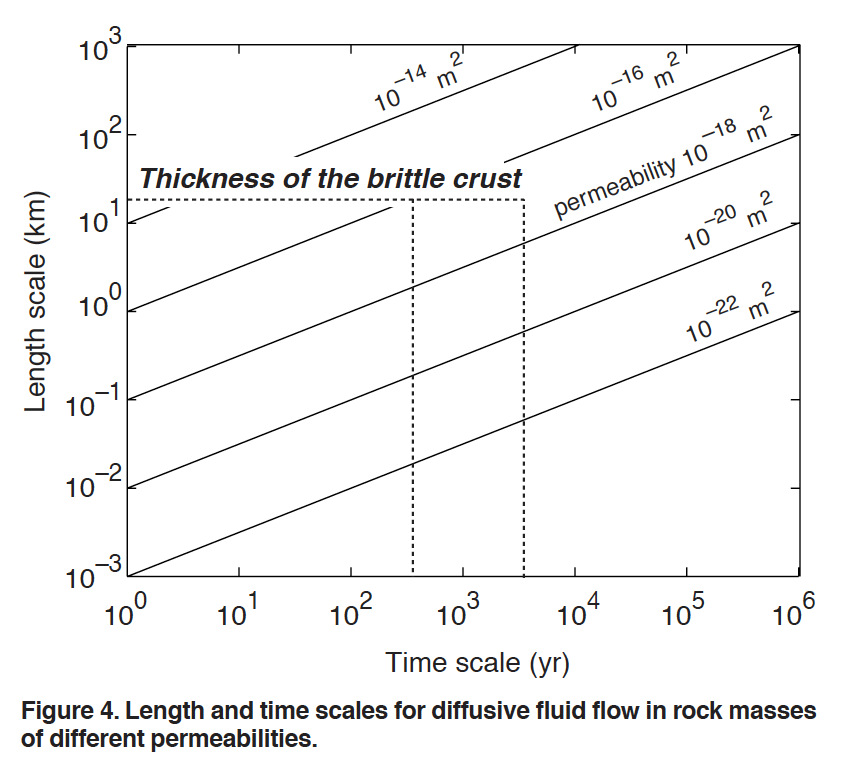
\includegraphics[width=0.7\linewidth]{images/4}
    \end{figure}
\end{frame}

\begin{frame}[fragile]{Questions and Discussions}
    \begin{itemize}
        \item The depth measurements are shallow, we can talk about induced seismicity but not about most faults?
        \item High permeability would imply what in terms of pore pressure?
        \item What is the relation between differential stress and fluid pressure?
        \item Characteristic length scale of faulting?
    \end{itemize}

\end{frame}
\end{document}

